%%  This is the main file to compile the document
\documentclass[12pt]{article}
\usepackage{setspace}
\usepackage{fullpage} %% better margin use
\usepackage[final]{graphicx}
\usepackage{xcolor,colortbl}
\usepackage{enumitem}
%\usepackage{subfig}
\usepackage{caption}
\usepackage{subfigure}
\usepackage{multirow}
\usepackage{amsmath}
\setdescription{leftmargin=\parindent,labelindent=\parindent}
\usepackage{units}
\usepackage{xfrac} %slanted fractions
\usepackage[colorlinks,linkcolor={red},citecolor={red}]{hyperref}
%\hypersetup[colorlinks, linkcolor=red, filecolor=red,  pagecolor=red,
%urlcolor=red]{hyperref}
\usepackage[version=4]{mhchem}

\graphicspath{{./figures/}{./figures/introduction/}{./figures/evaluations/}{./figures/experiment_overview/}{./figures/ratiocalculation/}{./figures/simulation/}{./figures/neutron_energy/}{./figures/energy_shape/}{./figures/isotopics/}{./figures/target_normalization/}{./figures/wraparound/}{./figures/efficiency/}{./figures/uncertainty/}{./figures/validations/}}


\newcommand{\verify}{\textbf{\textcolor{red}{Verify}}}
\newcommand{\etal}{\emph{et al.}}
\newcommand{\ie}{\emph{i.e.}}
\newcommand{\eg}{\emph{e.g.}}
\newcommand{\etc}{\emph{etc}}
\newcommand{\pu}[1][239]{$\mathrm{^{#1}}$Pu}
%\newcommand{\cf}[1][252]{$\mathrm{^{#1}}$Cf} 
\renewcommand{\u}[1][235]{$\mathrm{^{#1}}$U}
\newcommand{\hyd}[1][1]{$\mathrm{^{#1}}$H}  
\newcommand{\talpha}{$\alpha$}
\newcommand{\talphas}{$\alpha$s}
\newcommand{\ftpc}{fissionTPC}
\newcommand{\mev}{MeV}
\newcommand{\mus}{~$\mu$s}
\newcommand{\massunits}{\ensuremath{\mathrm{\mu g /cm^{2}}}}
\renewcommand{\textfraction}{0.15}
\renewcommand{\topfraction}{0.85}
\renewcommand{\bottomfraction}{0.65}
\renewcommand{\floatpagefraction}{0.6}

\newcommand{\HRule}{\rule{\linewidth}{0.5mm}}

%% ==============================================
%%  package for commenting
%%  documentation at: http://get-software.net/macros/latex/contrib/fixme/fixme.pdf
%% ==============================================
% use option 'final' to remove all comments
\usepackage[draft, inline, nomargin]{fixme}
\fxsetup{theme=color, mode=multiuser}
% this create a custom note command for a user
\FXRegisterAuthor{nb}{anb}{\color{blue}NB}      % creates \nbnote{} command
\FXRegisterAuthor{rv}{arv}{\color{red}RV}      % creates \rvnote{} command
 

\bibliographystyle{unsrt}






\begin{document}
%title page
\begin{titlepage}

\begin{center}

% Upper part of the page

\includegraphics[width=0.50\textwidth]{figures/PROSPECT_logo}\\[1cm]    

% Title
\HRule \\[0.4cm]
{\huge \bfseries Early Energy Scale Study for PROSPECT AD}
\HRule \\[1.5cm]

%\textsc{\Large LLNL-TR-732603-DRAFT}\\[1.5cm]

{\Large X. Zhang}\\
\emph{\Large PROSPECT Collaboration}\\


\vfill
% Bottom of the page
{\large \today}

\end{center}

\end{titlepage}
\newpage


\newpage
\tableofcontents{}

\newpage
\section*{Working Notes}

Relevant DocDB entries
\begin{itemize}

\item First look at gamma source calibrations

\item First look at $^{12}$B in full detector

\item Energy scale study with combined calibrations on PROSPECT AD



\end{itemize}

\newpage

\section{Introduction}
\label{sec:intro}
The first physics result of PROSPECT will show the reconstructed prompt energy spectrum of IBD events, perform model independent spectral comparison between baselines for oscillation analysis, and the data vs. model comparison of reconstructed prompt spectrum.

The reconstructed energy of particle events in detector is naturally different from the energy deposit by the particles because of detector response. 
It is vital to characterize the detector response with correct  nonlinearity of energy response and energy resolution to
\begin{itemize}
    \item Supply accurate detector response model through MC with correct key values.
    \item Quantify the systematic uncertainty in energy response. 
    \item Tweak the data calibration constants.
\end{itemize}

In this study, we utilized the gamma source calibration and ambient calibration to understand the absolute detector response, including nonlinearty induced by the Birk's law quenching and Cherenkov radiation of scintillator, the energy resolution that is contributed by the detector geometry and photon statistics, and absolute energy scale caused by calibration pressumption of n-capture electron equivalent energy.
%TODO add neutron capture and alpha energy response when they are available.

\section{Calibrations}
In early calibration runs, the sources $^{137}$Cs, $^{22}$Na and $^{60}$Co were available to us.
Table \ref{tab:src_table} shows the decay and particle energy of the sources..
\begin{table}
    \centering
    \begin{tabular}{c|c|c}
        Source & Decay Type & Energy[MeV]\\
        $^{137}$Cs  & $\beta^-$   & $0.662 \gamma$\\
        $^{22}$Na   & $\beta^+$   & $1.274 \gamma + 2\times0.511$ \\
        $^{60}$Co   & $\beta^-$   & $1.17 + 1.33 \gamma$
    \end{tabular}
    \caption{Calibration source utilized}
    \label{tab:src_table}
\end{table}

Each source was inserted through calibration tube by time belt and deployed close to the center of detector.
Once in position, the each energy scale calibration run last for 10 minutes.
To read the calbiration data, PROSPECT2x analysis package \cite{P2X} is used to reconstruct the gamma energy of clusters in the full detector and compton scattering energy deposited into single segments. 
Before the calibration runs, a half-hour long reactor off background data is collected for background subtraction. 
The gamma calibration spectra is shown in Figure \ref{fig:gammacalib}.

\begin{figure}[h!]
\centering
\subfigure[The gamma energy distribution from $^{137}$Cs calibration.]{\label{fig:a}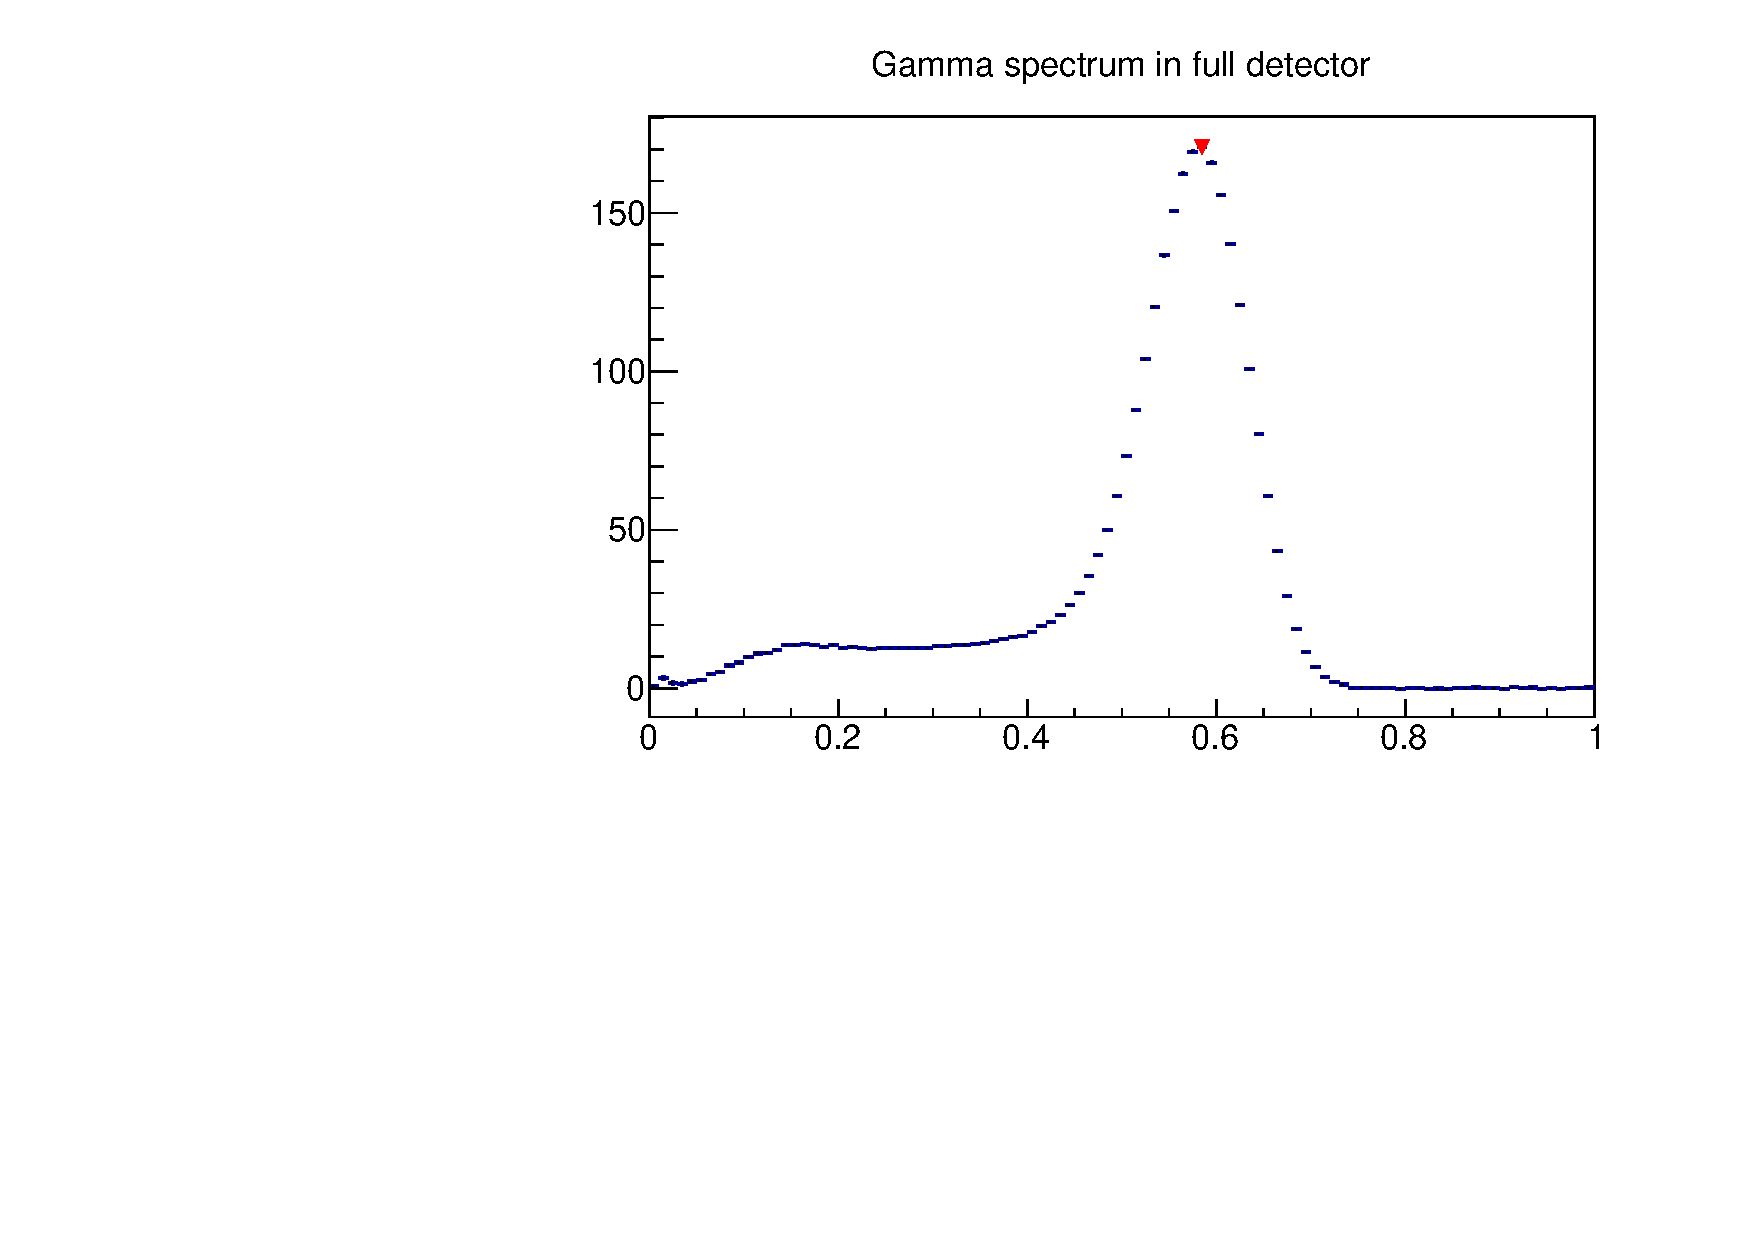
\includegraphics[width=60mm]{figures/hCs137.pdf}}\quad
\subfigure[The gamma energy distribution from $^{22}$Na calibration.]{\label{fig:b}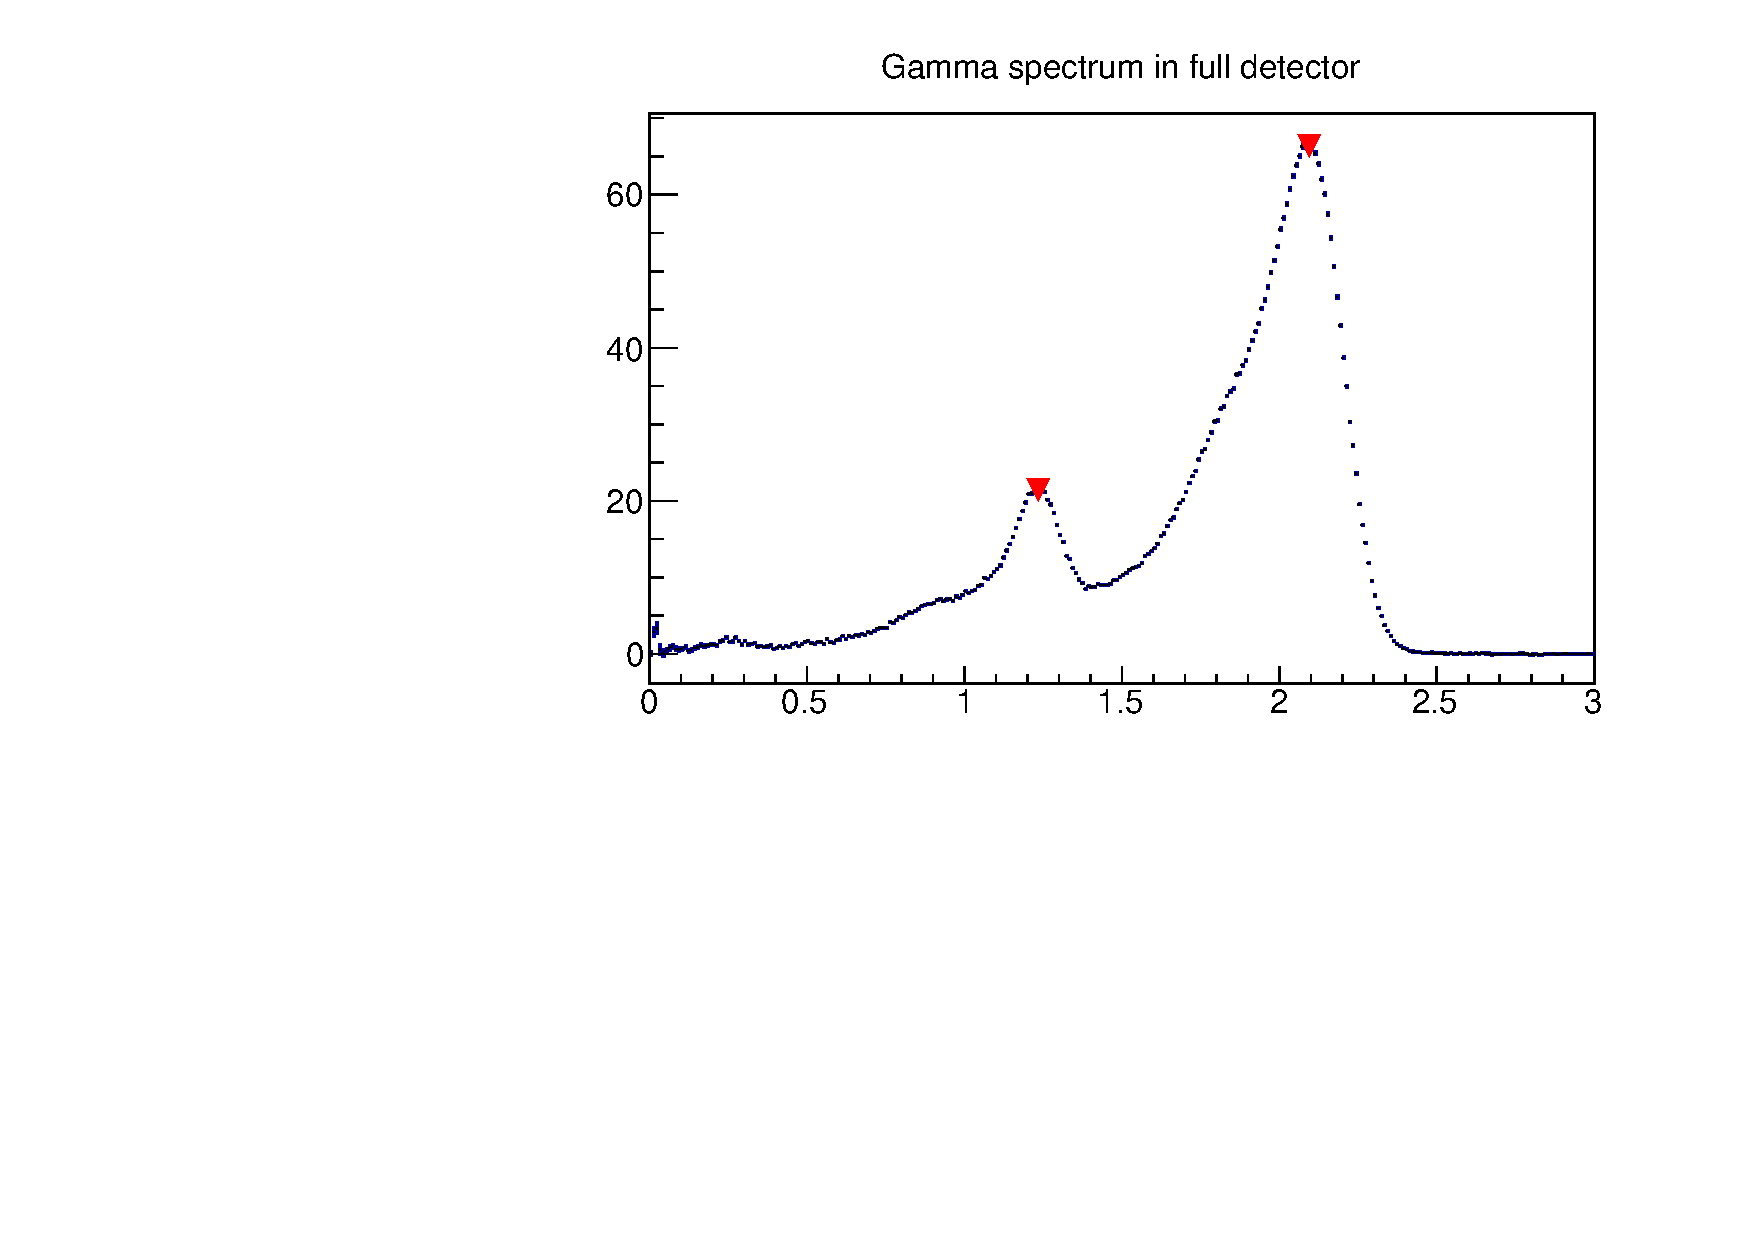
\includegraphics[width=60mm]{figures/hNa22.pdf}} \\
\subfigure[The gamma energy distribution from $^{60}$Co calibration.]{\label{fig:b}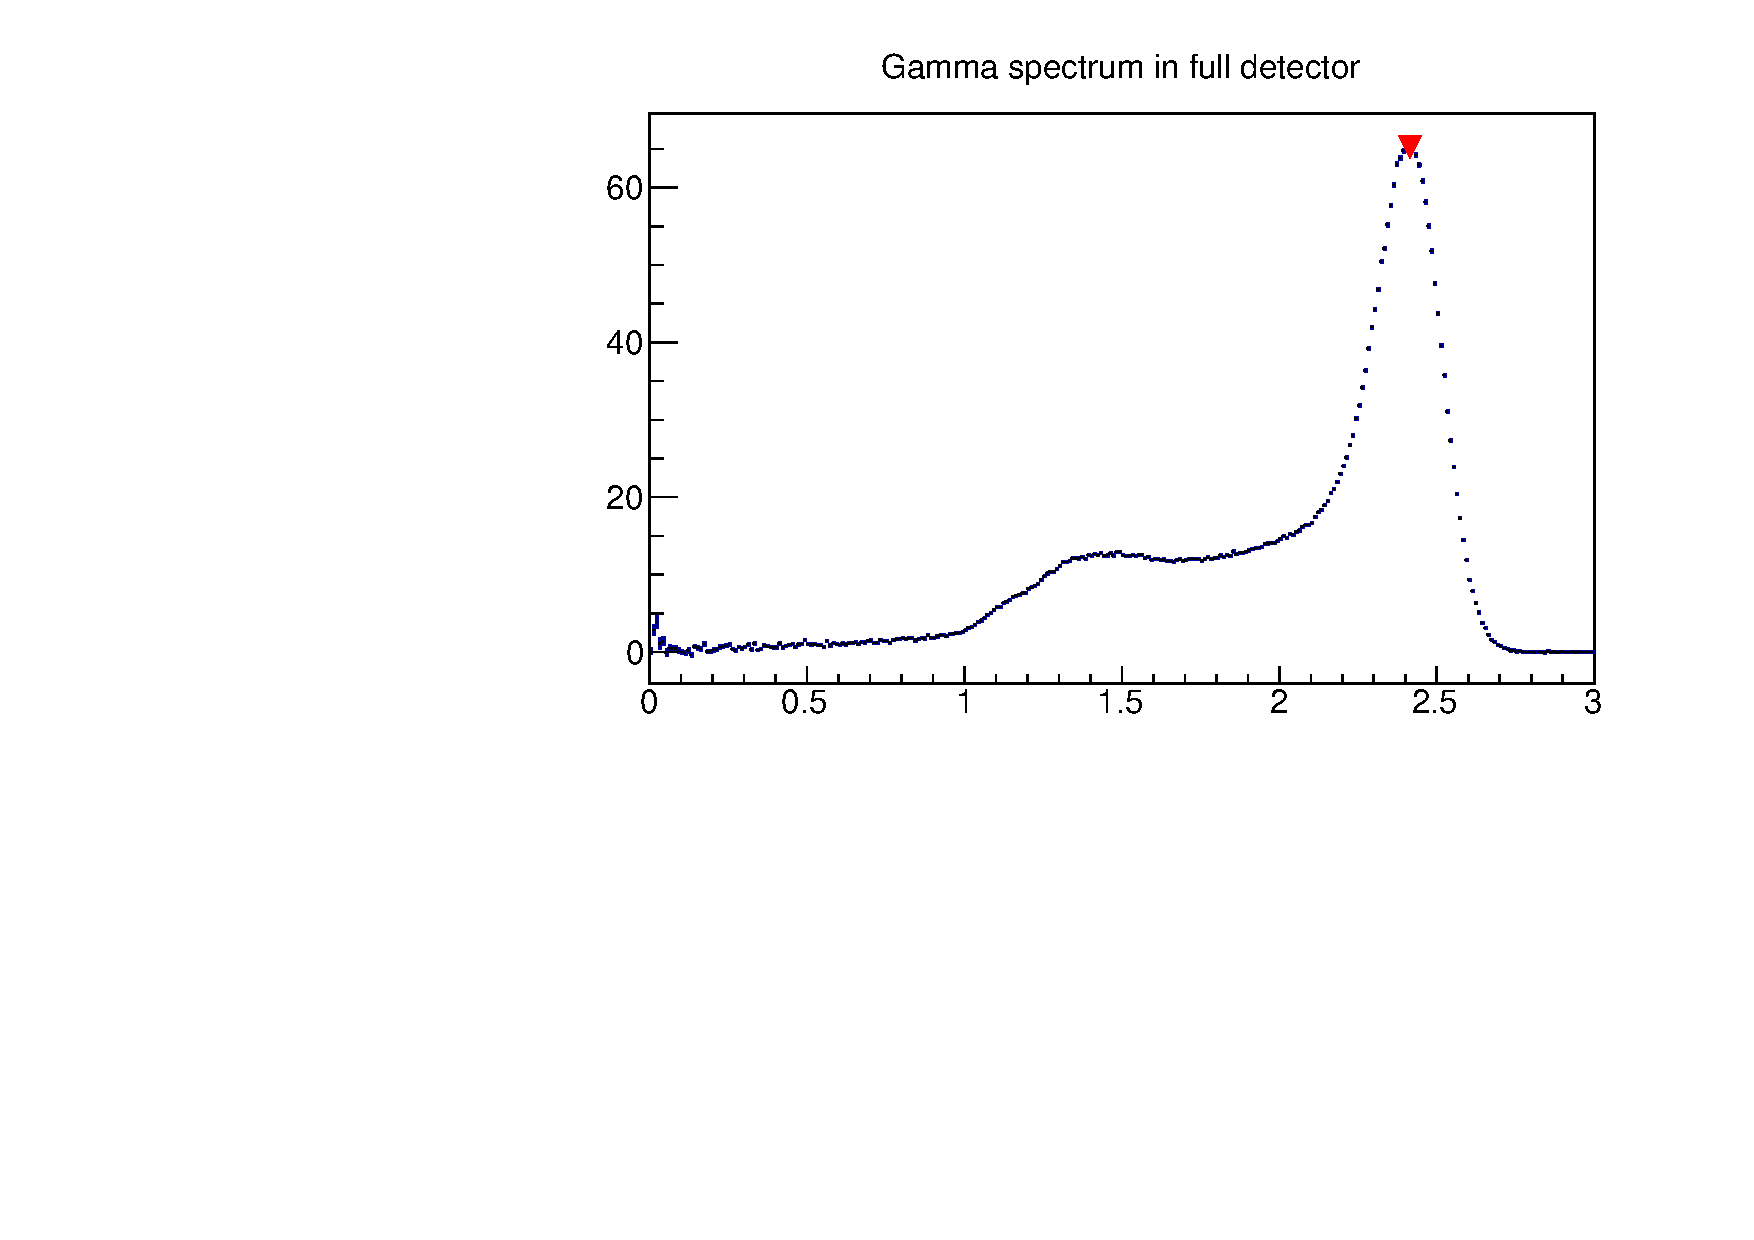
\includegraphics[width=60mm]{figures/hCo60.pdf}} 
\caption{The gamma spectra of calibration sources.}
\label{fig:gammacalib}
\end{figure}

The $^{12}$B is an ambient electron source in PROSPECT detector that is induced by cosmogenic neutron with $^{12}$C(n, p)$^{12}$B interaction.
The cross section of this interaction is $\sim 0.01$ barn. 
It is a valued calibration source to demonstrate the correct scale of reconstructed energy of IBD events.
To acquire $^{12}$B events in PROSPECT, we collected recoil coincident ionization events by allowing the single-cell-hit recoil events in 0.7 to 10 MeVee range that followed by less than 3-cell-hit electron candidates with energy less than 20 MeV. 
In the procedure above, we used PSD to separate recoil and ionization events. The life time is 29.0 ms, shown in Figure \ref{fig:lifetime}. 
The prompt to delay distance is fitted with guassian distribution, the best fit  stardard deviation = 2.99 cm, shown in Figure \ref{fig:distance}. 
During the 25.4 days of reactor off period, we collected about 11656 events of $^{12}$B decay. 
The reconstructed spectrum of $^{12}$B electron is shown in \ref{fig:B12}.
\begin{figure}[h!]
\centering
\subfigure[The delay-prompt time difference of $^{12}$B candidates ]{\label{fig:lifetime}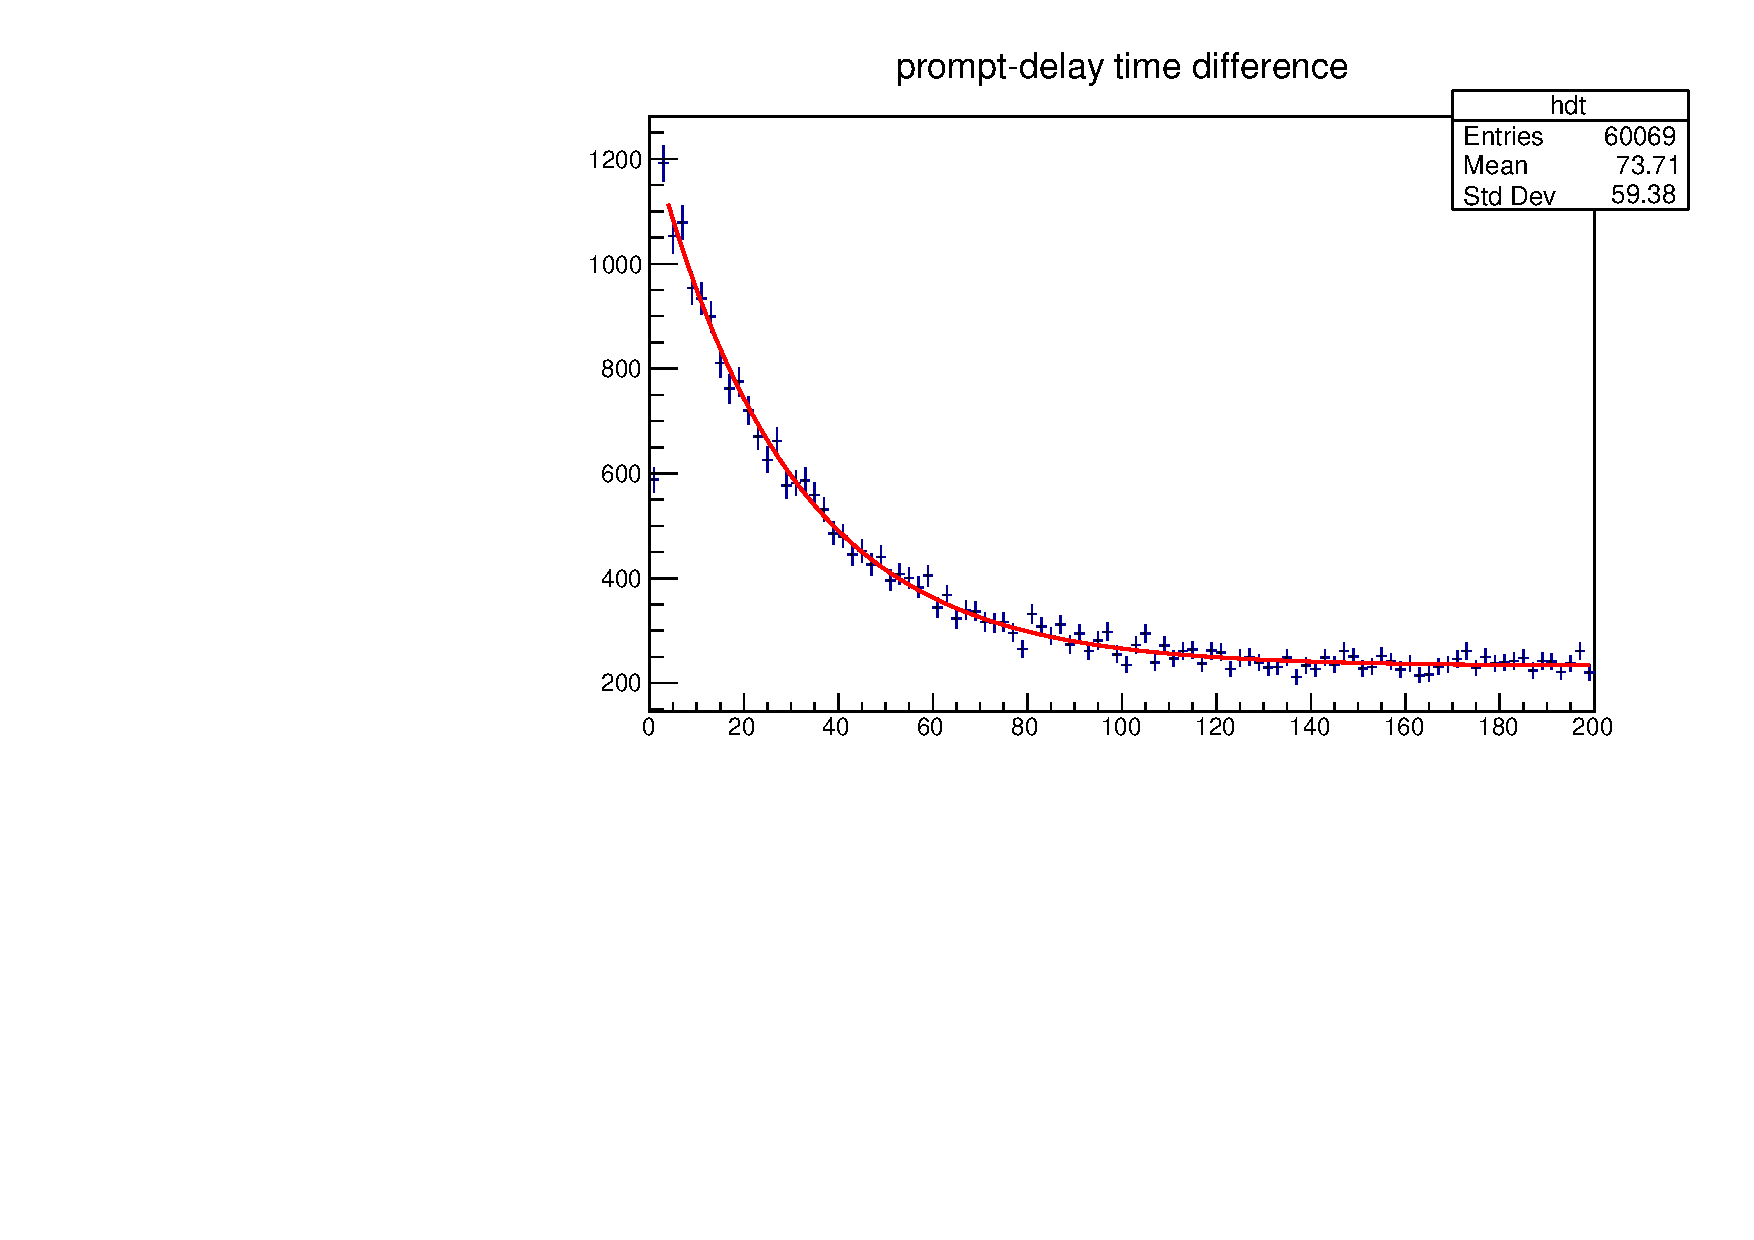
\includegraphics[width=60mm]{figures/lifetime.pdf}}\quad
\subfigure[The delay-prompt distance of $^{12}$B candidates]{\label{fig:distance}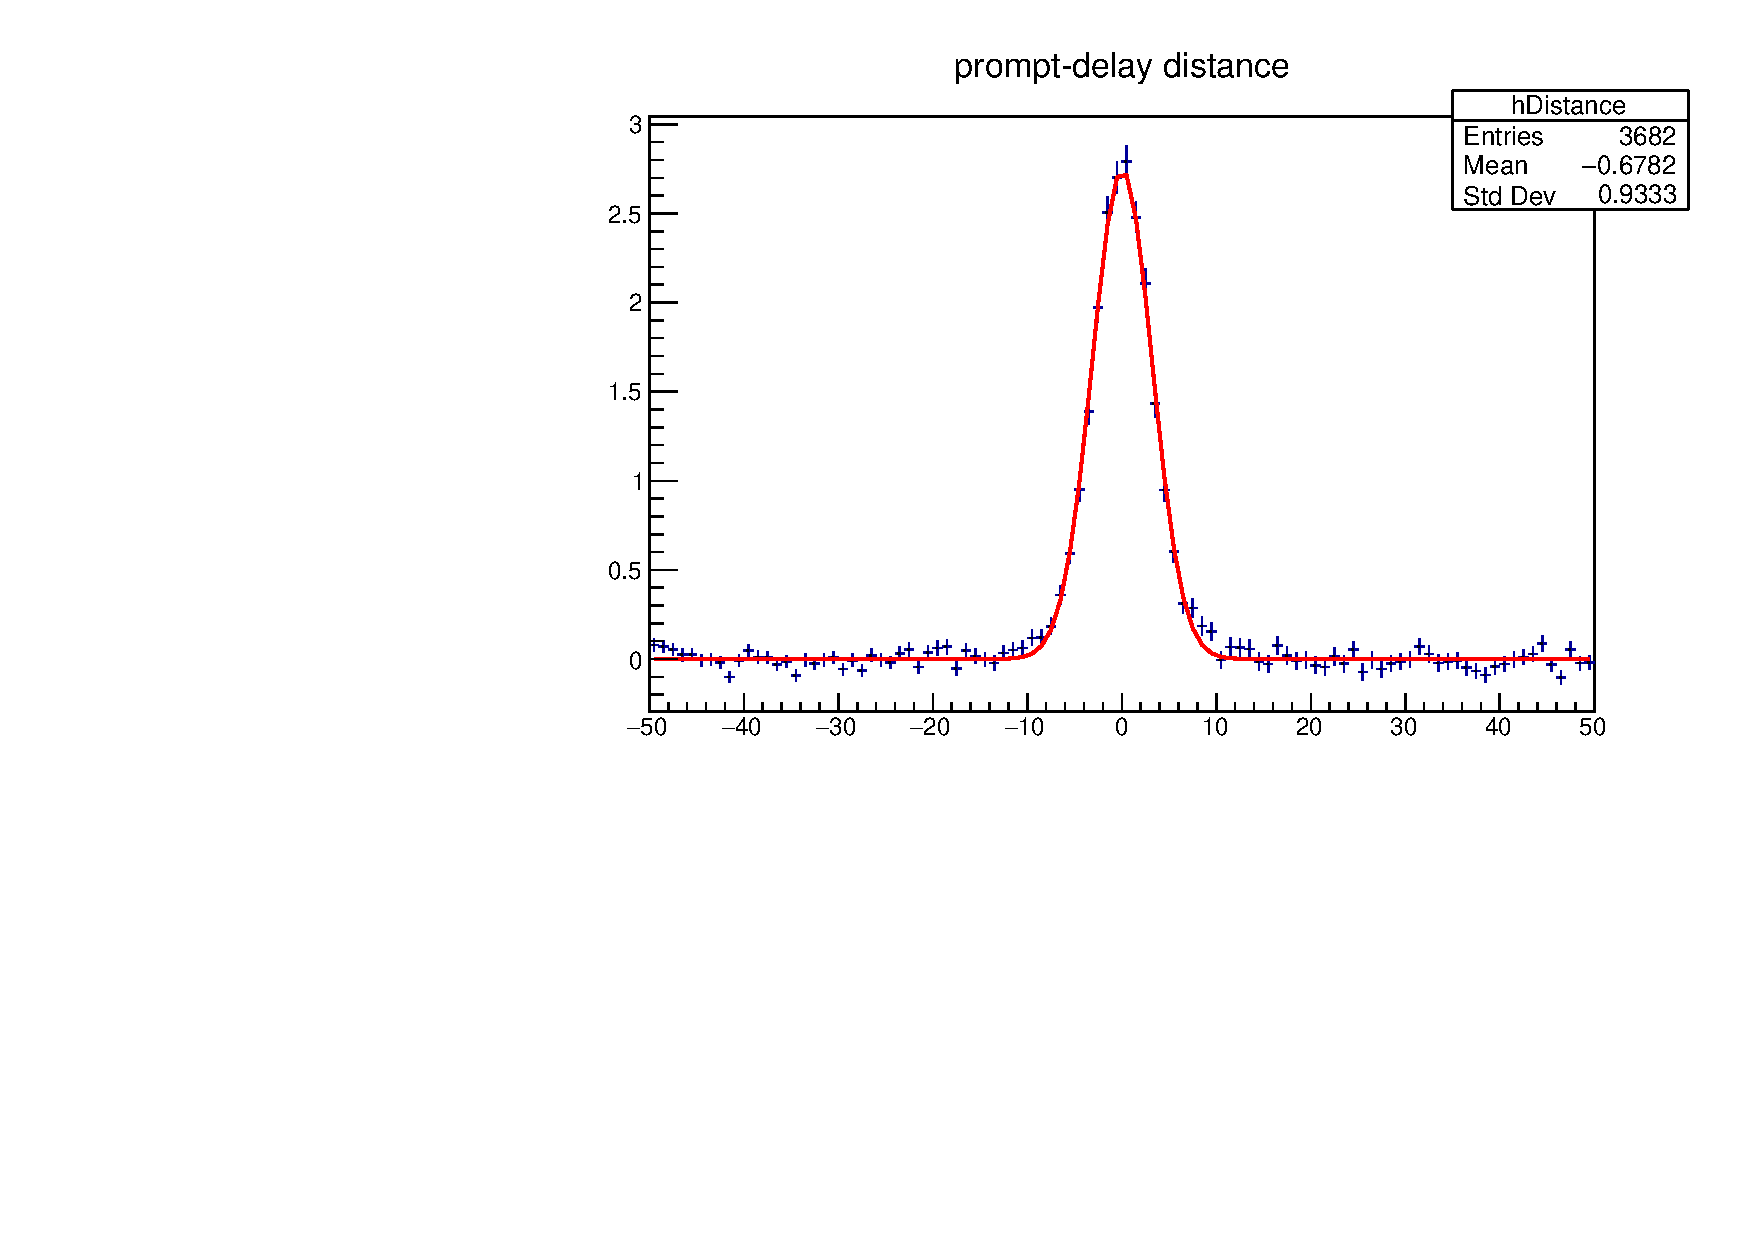
\includegraphics[width=60mm]{figures/distance.pdf}} \\
\subfigure[$^{12}$B spectrum.]{\label{fig:B12}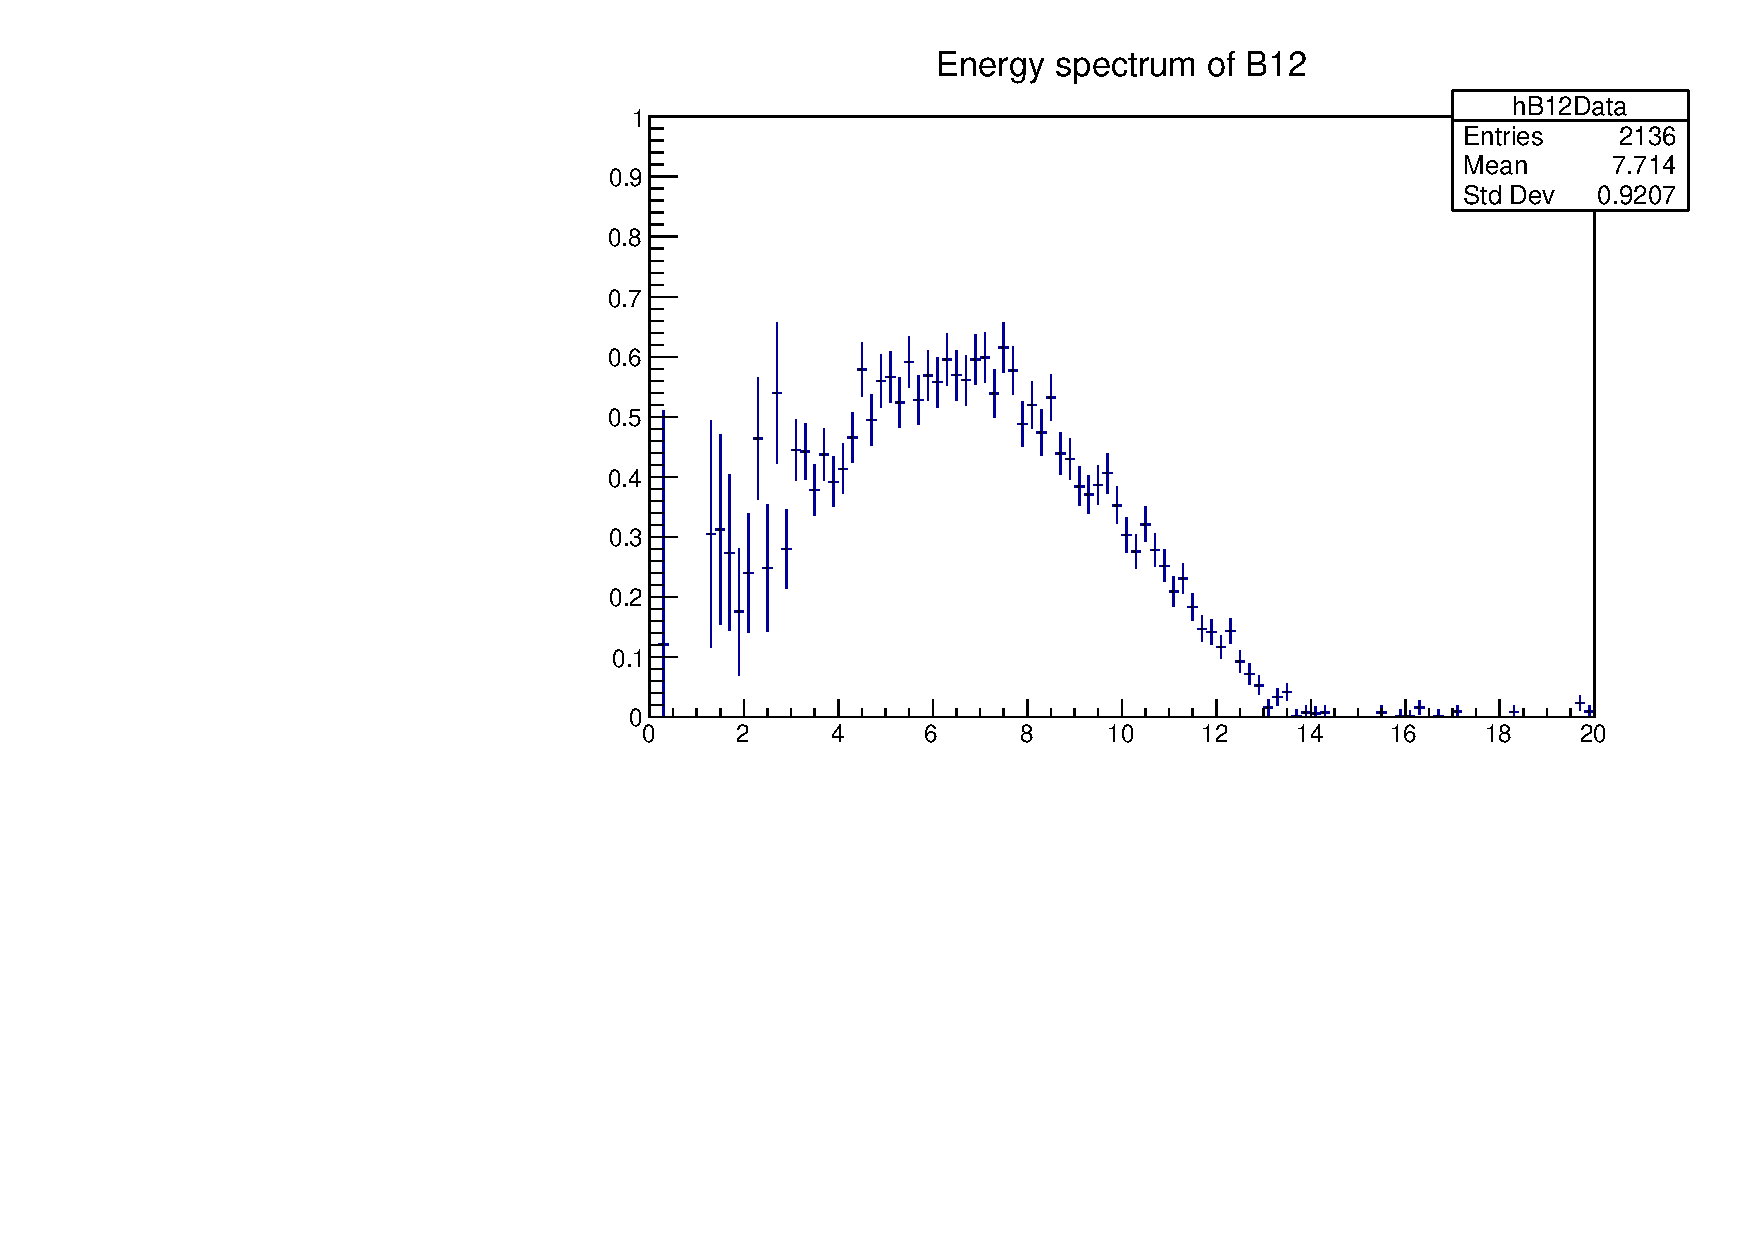
\includegraphics[width=60mm]{figures/hB12.pdf}} 
\caption{The observation of $^{12}$B events in PROSPECT.}
\label{fig:B12plots}
\end{figure}


\section{Monte-Carlo vs. Data Comparisons}
The purpose of the comparison between Monte-Carlo and calibration data is to characterize the detector energy response, so we are able to provide trust worthy IBD prompt energy spectrum model with precisely tweaked detector response. 
The detector response includes the energy scale contributed by the nonlinearity of liquid scintillator (LS), the relative energy scale affected by detector geometry and resolution of reconstructed energy mainly influenced by the photon statistics of scintillator. 
Thus, the Birk’s constant in detector $k_B$, the detect efficiency of Cherenkov light $k_{C}$, the absolute energy scale and the energy dependent resolution are the terms we needed to search precisely.

The PROSPECT-G4 simulation package \cite{PG4} was utilized to generate all of the calibration sources with the same configuration as calibration data. 
The nonlinearity from Birk’s quenching effect of scintillator and Cherenkov radiation from induced by electron was simulated by PROSPECT-G4. 
The energy resolution caused by photon statistics and potential absolute energy scale were applied on the MC generated energy spectrum. 

\subsection{Nonlinearity}
The energy response of LS is mainly affected by the Birk’s law quenching and Cherenkov radiation. 

The Birk’s law is a empirical function of the light yield per track length:
\begin{equation}
    \frac{dL}{dx} = \frac{\frac{dE}{dx}}{1+k_B\frac{dE}{dx}},
\end{equation}
where $k_B$ is the Birk's constant which is a property of LS. 
It represents the quenched reconstructed energy in LS, a nonlinear energy loss caused by particle-molecule interaction. 
In MC, we  simulate the quenching effect by multiplying energy difference in between particle scatters with a Birk's factor:
\begin{equation}
   \frac{1}{1+k_B\frac{dE}{dx}}.
   \label{eql:birks}
\end{equation}

%TODO add image indicating how Birk's constants affect the reconstruct energy.

The Cherenkov radiation is the light emitted as a charged particle traveling faster than the phase velocity of light in a medium. 
The molecules in the medium are polarized along the particle track, when the particle is faster than light, the electromagnetic field of molecule depolarization can add up as coherent light emission. 
The number of photon generated along the particle track can be expressed as:
\begin{equation}
    \frac{d^2N}{dxd\lambda} = \frac{2\pi\alpha z^2}{\lambda}\left(1- \frac{1}{\beta^2n^2(\lambda)}\right),
\end{equation}
where $N$ is number of photon, $\alpha$ is a fine structure constant, $z$ is the particle's electric charge, $\beta$ is the speed of the particle and $n(\lambda)$ is index of refraction.
In MC processing, we collected the energy emitted from the Cherenkov radiation as the summed energy of detected Cherenkov photons. 
We also assumed the LS's index of refraction remains same against wavelengths in 200-700 nm range.
The particle energy loss in Cherenkov radiation is negligible.

To simply model the detector energy scale, we adjusted the Birk's constant $k_B$ in equation \ref{eql:birks} and the detect efficiency of Cherenkov light $k_C$ to search the best-fit value with data.

%TODO add image to indicate how cherenkov affect the reconstructed energy.

\subsection{Energy Resolution}
The reconstructed resolution is a function of energy:
\begin{equation}
    \frac{\sigma}{E} = \sqrt{a^2 + \frac{b^2}{E}+\frac{c^2}{E^2}},
\end{equation}
where $a$ is affected by the detector geometry, $b$ is from the photon statistics (PE/MeV) and $c$ for the quantum efficiency of PMTs.

\subsection{Other Energy Scale Factors}
The reconstructed energy scale was initially based on the assumption that $n$ captured by $^6$Li yield 0.55 MeVee in detector. 
The deviation of true electron equivalent energy to this estimation can induce a constant energy scale throughout the all energy. 
This absolute energy scale, as a fitting parameter, was searched together with other energy response parameters.

The zero length encoding (ZLE) threshold was applied during data acquisition, requiring each ADC channel to record signals that are only above specific magnitude. 
By excluding electronic noise, this threshold also affect the energy scale nonlinearly by excluding small deposition of energy in some segments in multi-hit events. 
To ensure MC being precisely compared to data, ZLE threshold was simulated in PROSPECT2x's CalcDetectorPulseResponse program.

\section{$\chi^2$ Test}
The MC calibration spectrum was compared with data by $\chi^2$ test. 
We generated a list of calibration MC with specific values of $k_B$ and $k_C$. 
The tweaked MC spectra were then scaled with a constant energy scale and smeared with the resolution as the function of energy.
To exclude the influence of ZLE threshold to reconstructed energy, we first compared the Compton scattering energy of gamma collected by single segment. 
The range of data vs. MC fitting for gamma calibration source were selected from 0.2 MeV to the edge of energy distribution. 
The range for $^{12}$B spectrum is 3 to 13.5 MeV. 
At last, the summed $\chi^2$ value for all calibration sources listed above was minimized by MINUIT to search for best-fit parameters. 
Based on our knowledge to the detector, the $a$ and $c$ are currently assumed to be zero. 

To simplify the simulation, the amount of MC events was irrelevant to the event rates of calibration data. 
However, the MC was normalized to match the integral of data event rate in the energy range of interest. 

%TODO change the values to the real best fit. 
The lowest $\chi^2/NDF = 207.11/499$ with the parameters: $k_B = 0.107 \pm 0.001$ mm/MeV , $k_C = 89 \pm 1\%$, $\beta_{rec} = 101.2 \pm 0.1\%$ and $b = 5.49\%$. The result of the fit can be shown in Figure \ref{fig:goodfit} and \ref{fig:chi2}.

\begin{figure}[h!]
\centering
\subfigure[Best-fit MC-data for $^{137}$Cs calibration.]{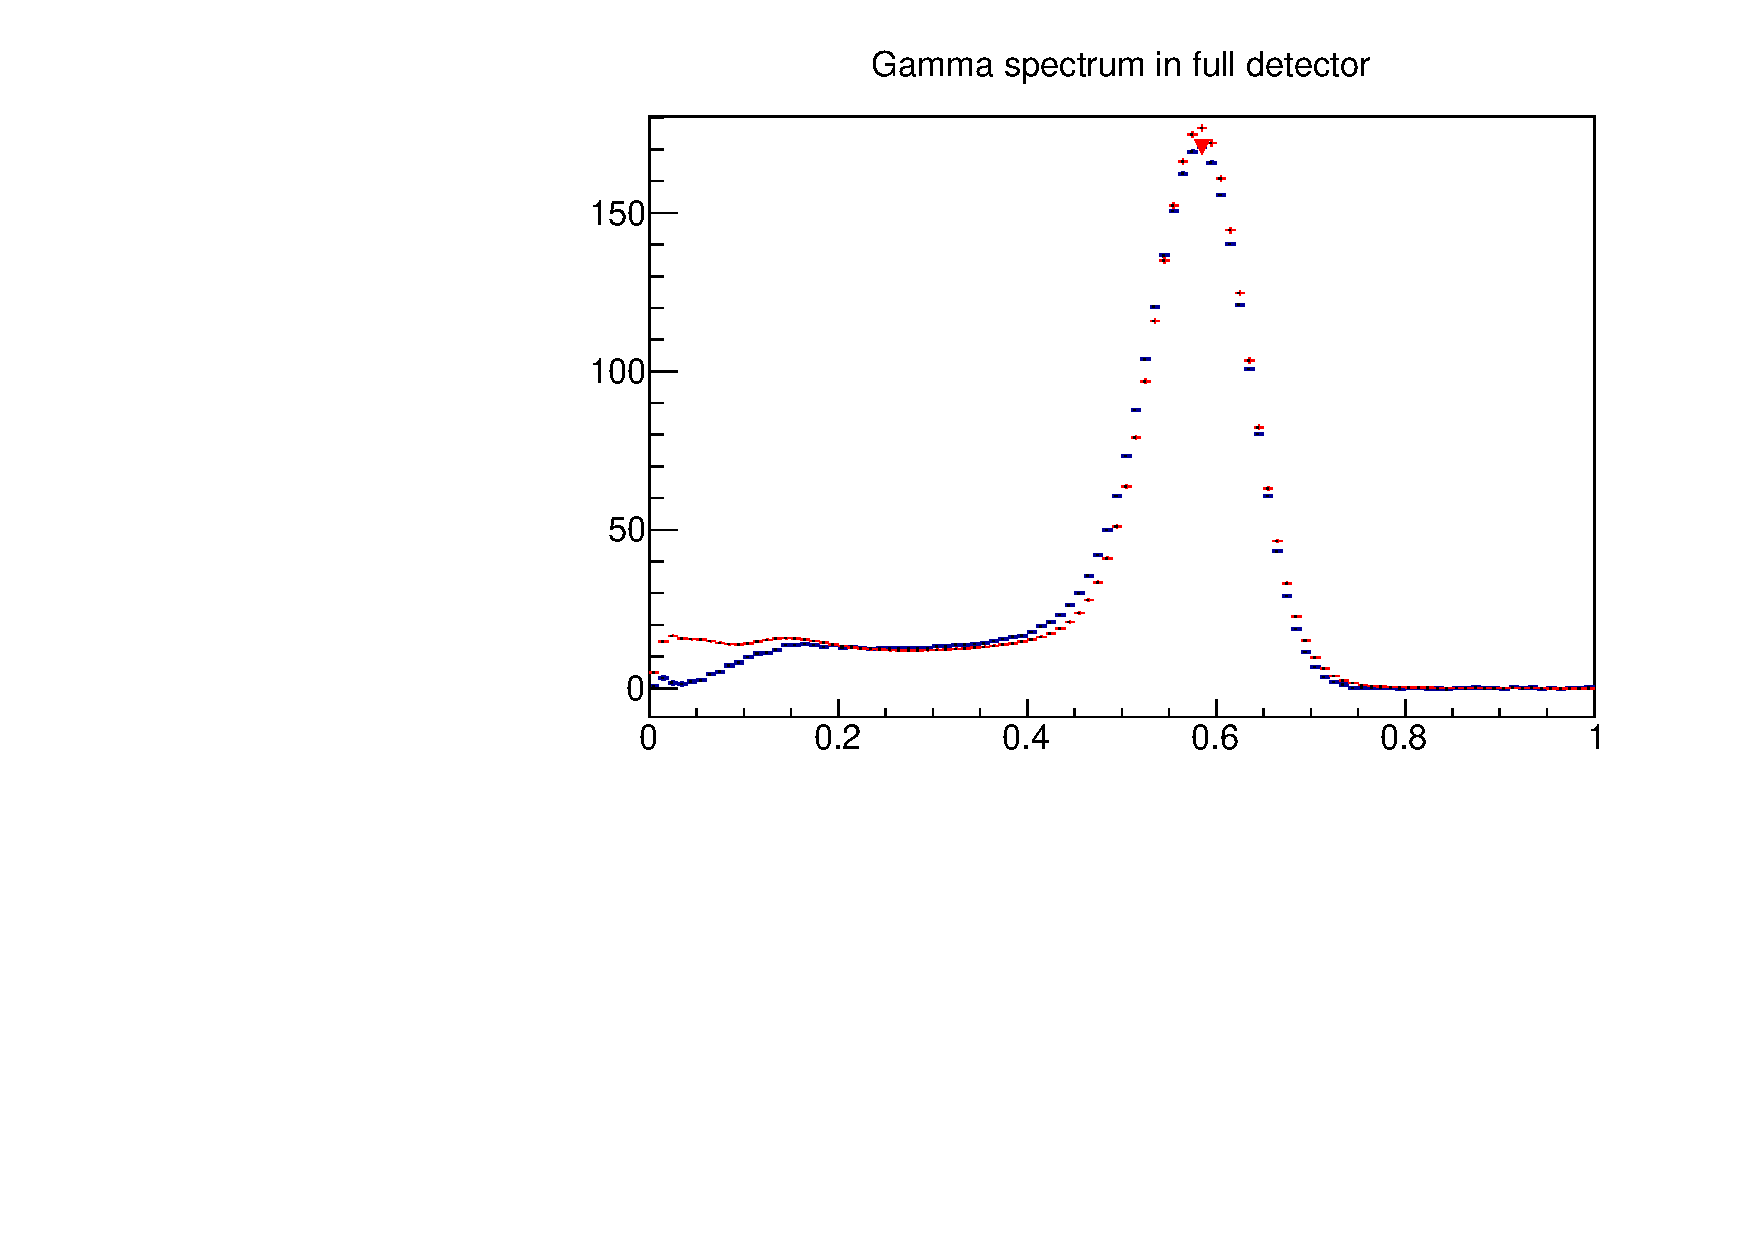
\includegraphics[width=60mm]{figures/hCs137match.pdf}}\quad
\subfigure[Best-fit MC-data for $^{22}$Na calibration.]{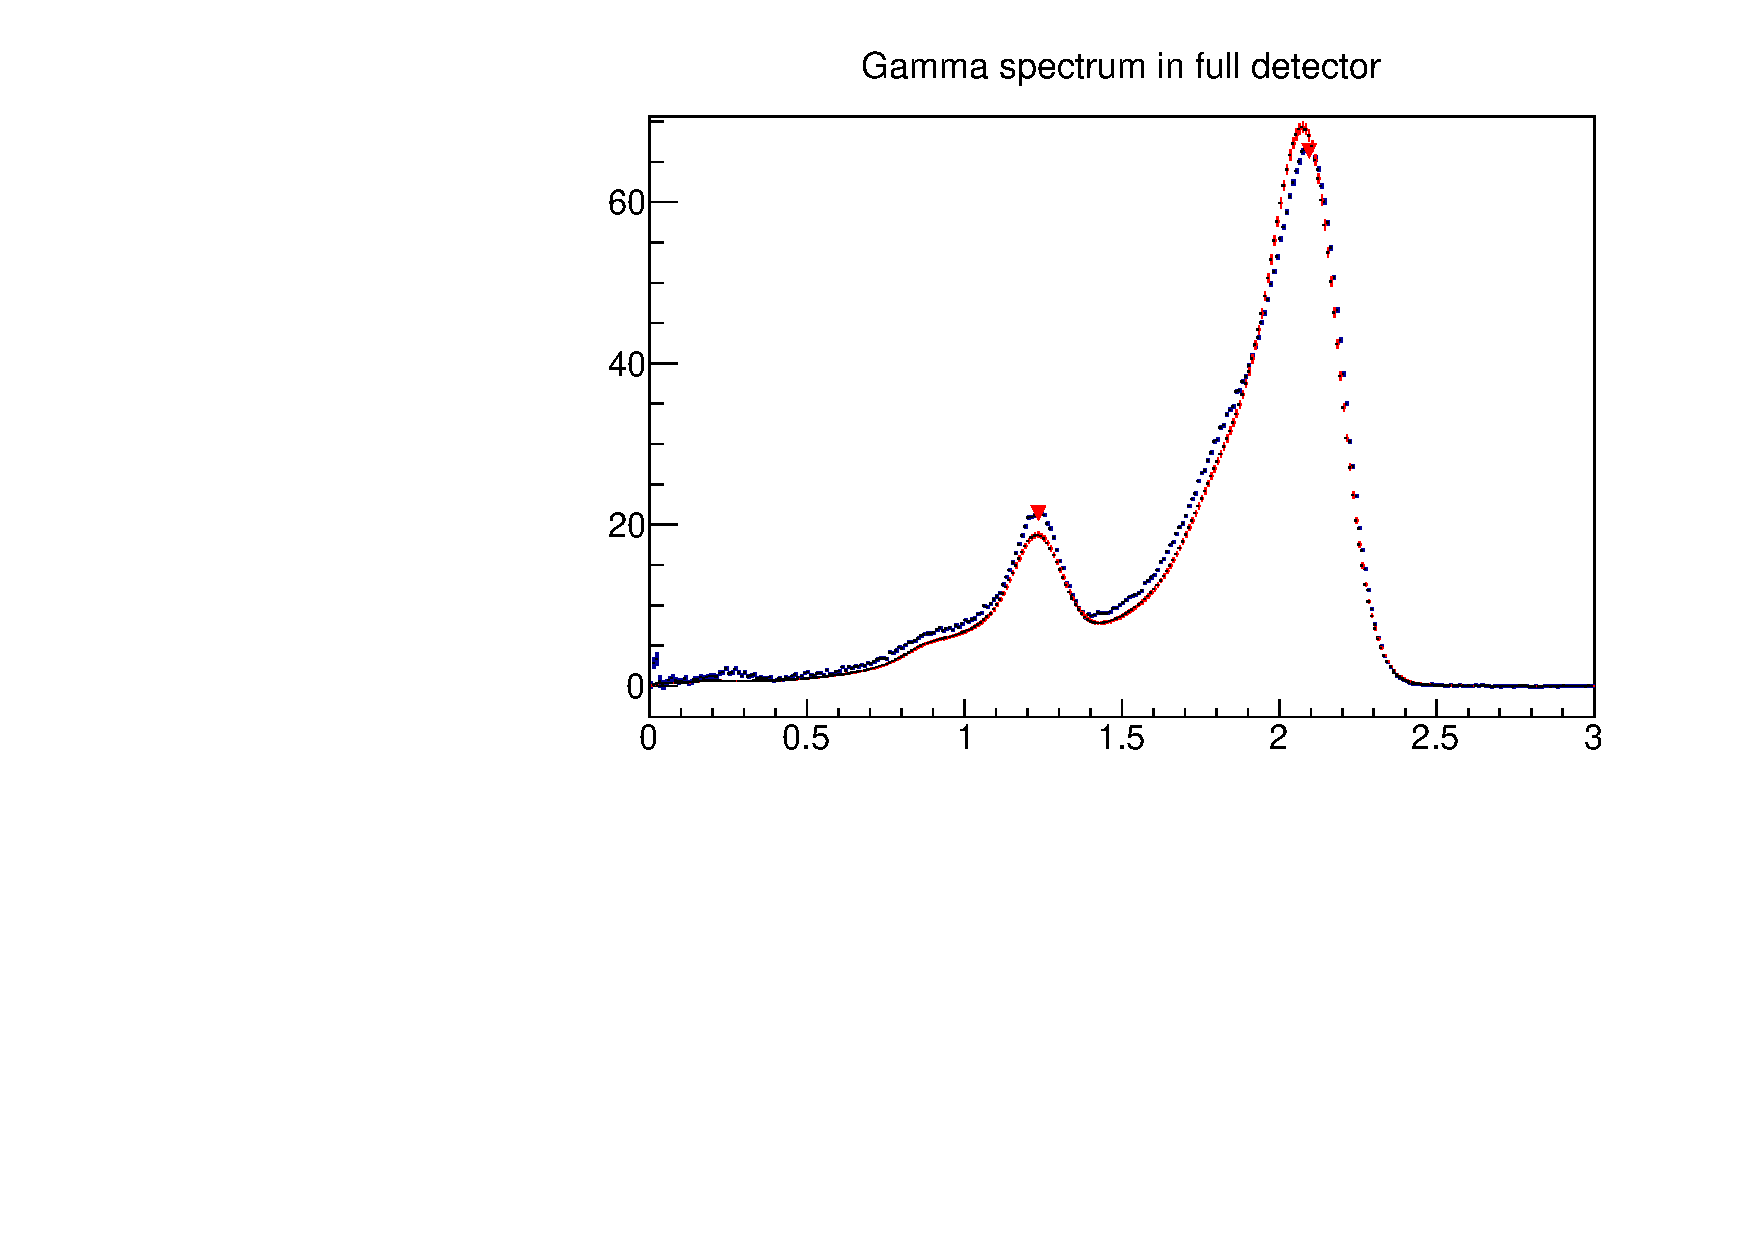
\includegraphics[width=60mm]{figures/hNa22match.pdf}} \\
\subfigure[Best-fit MC-data for $^{60}$Co calibration.]{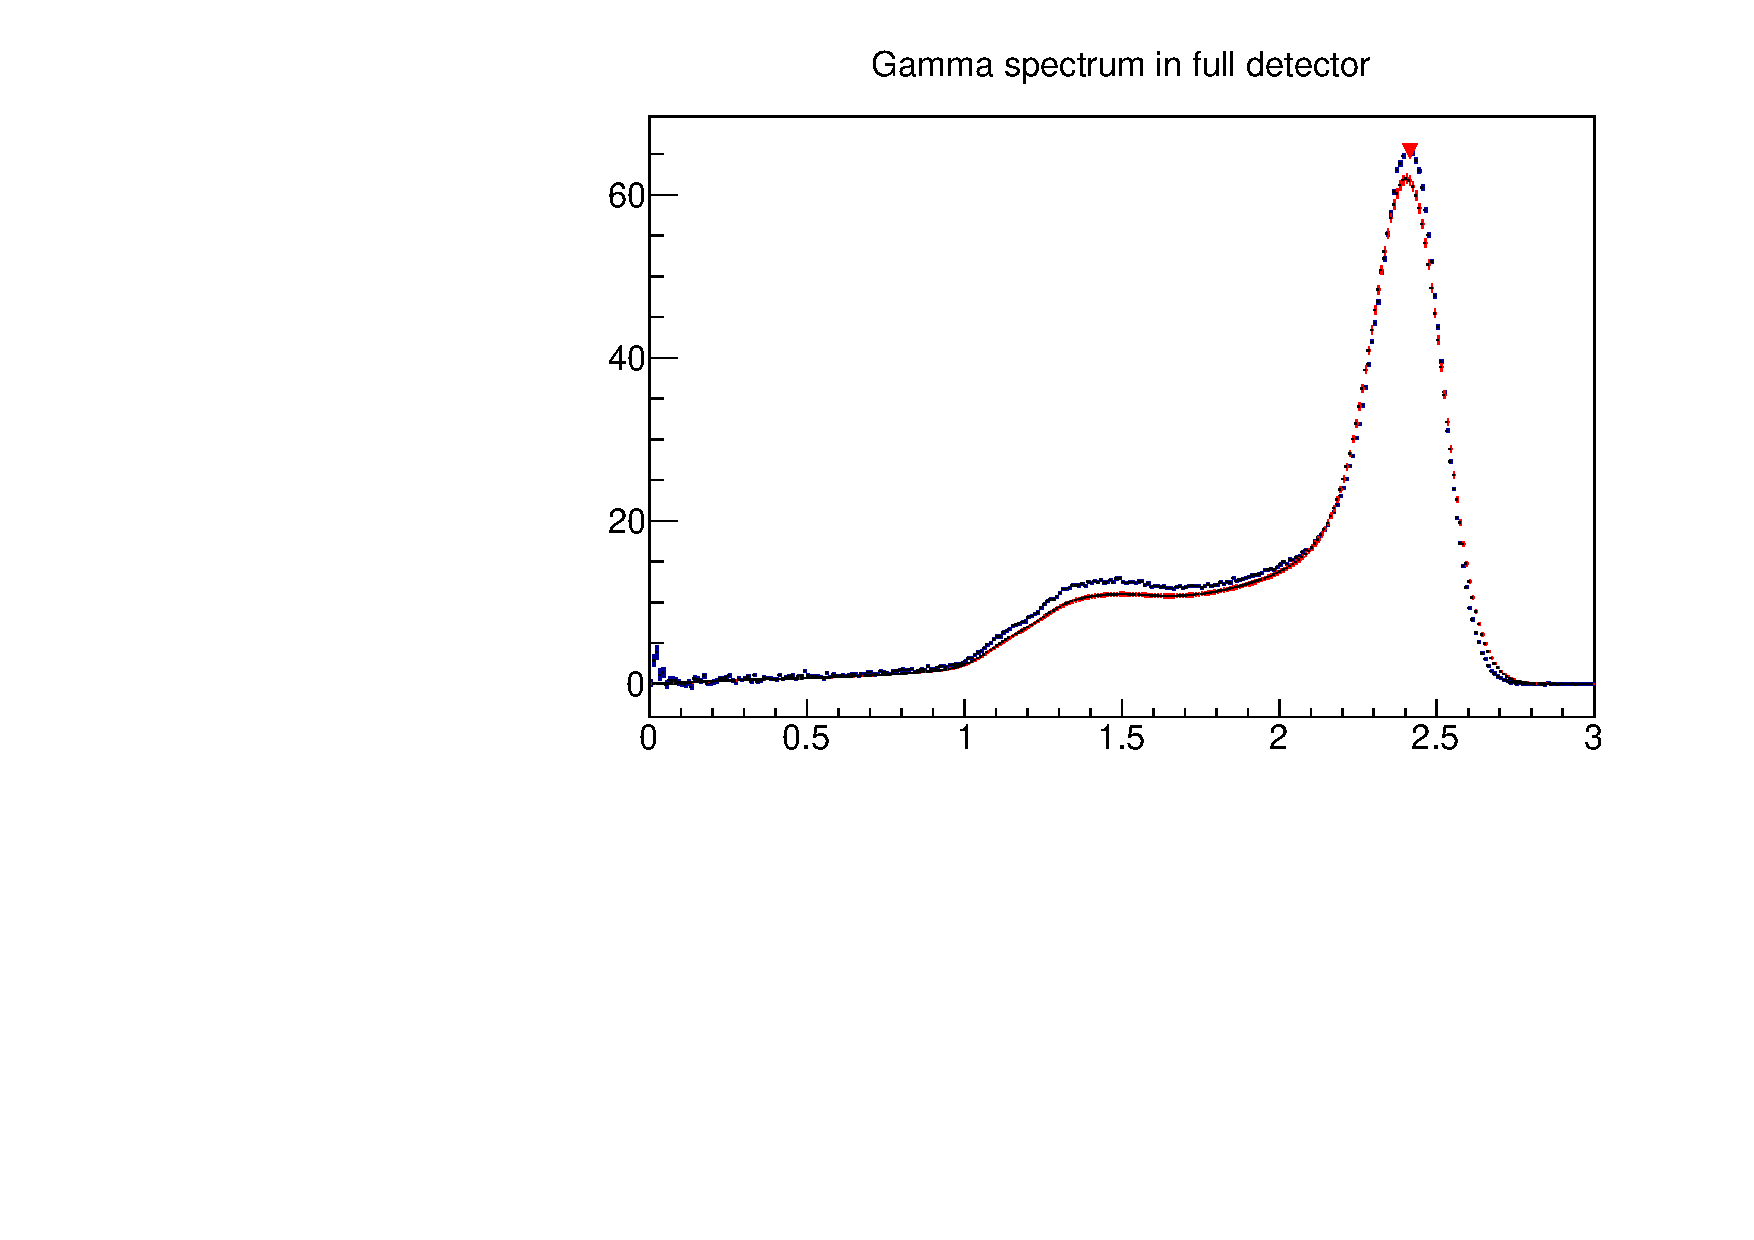
\includegraphics[width=60mm]{figures/hCo60match.pdf}} \quad
\subfigure[Best-fit MC-data for $^{12}$B]{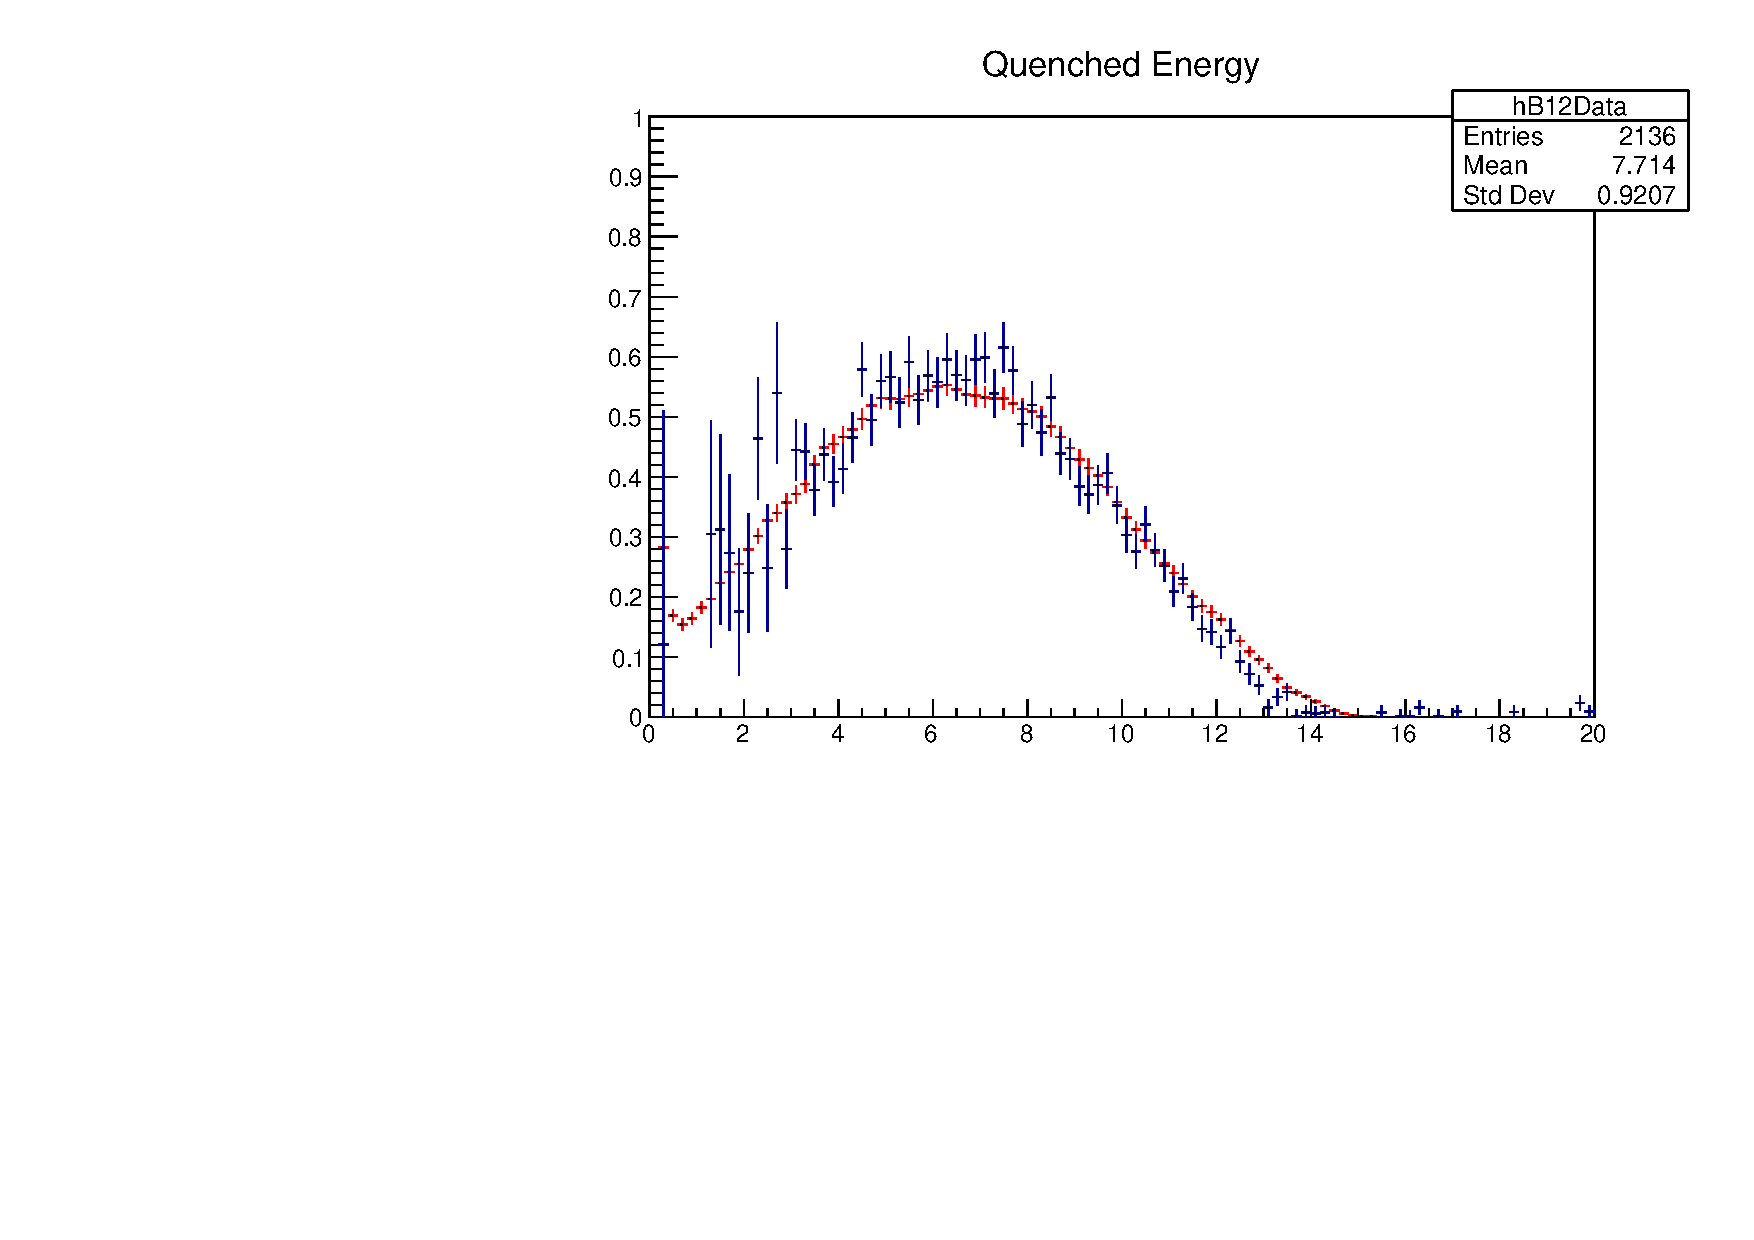
\includegraphics[width=60mm]{figures/hB12match.pdf}} 
\caption{The best fit results.}
\label{fig:goodfit}
\end{figure}

\begin{figure}[h!]
\centering
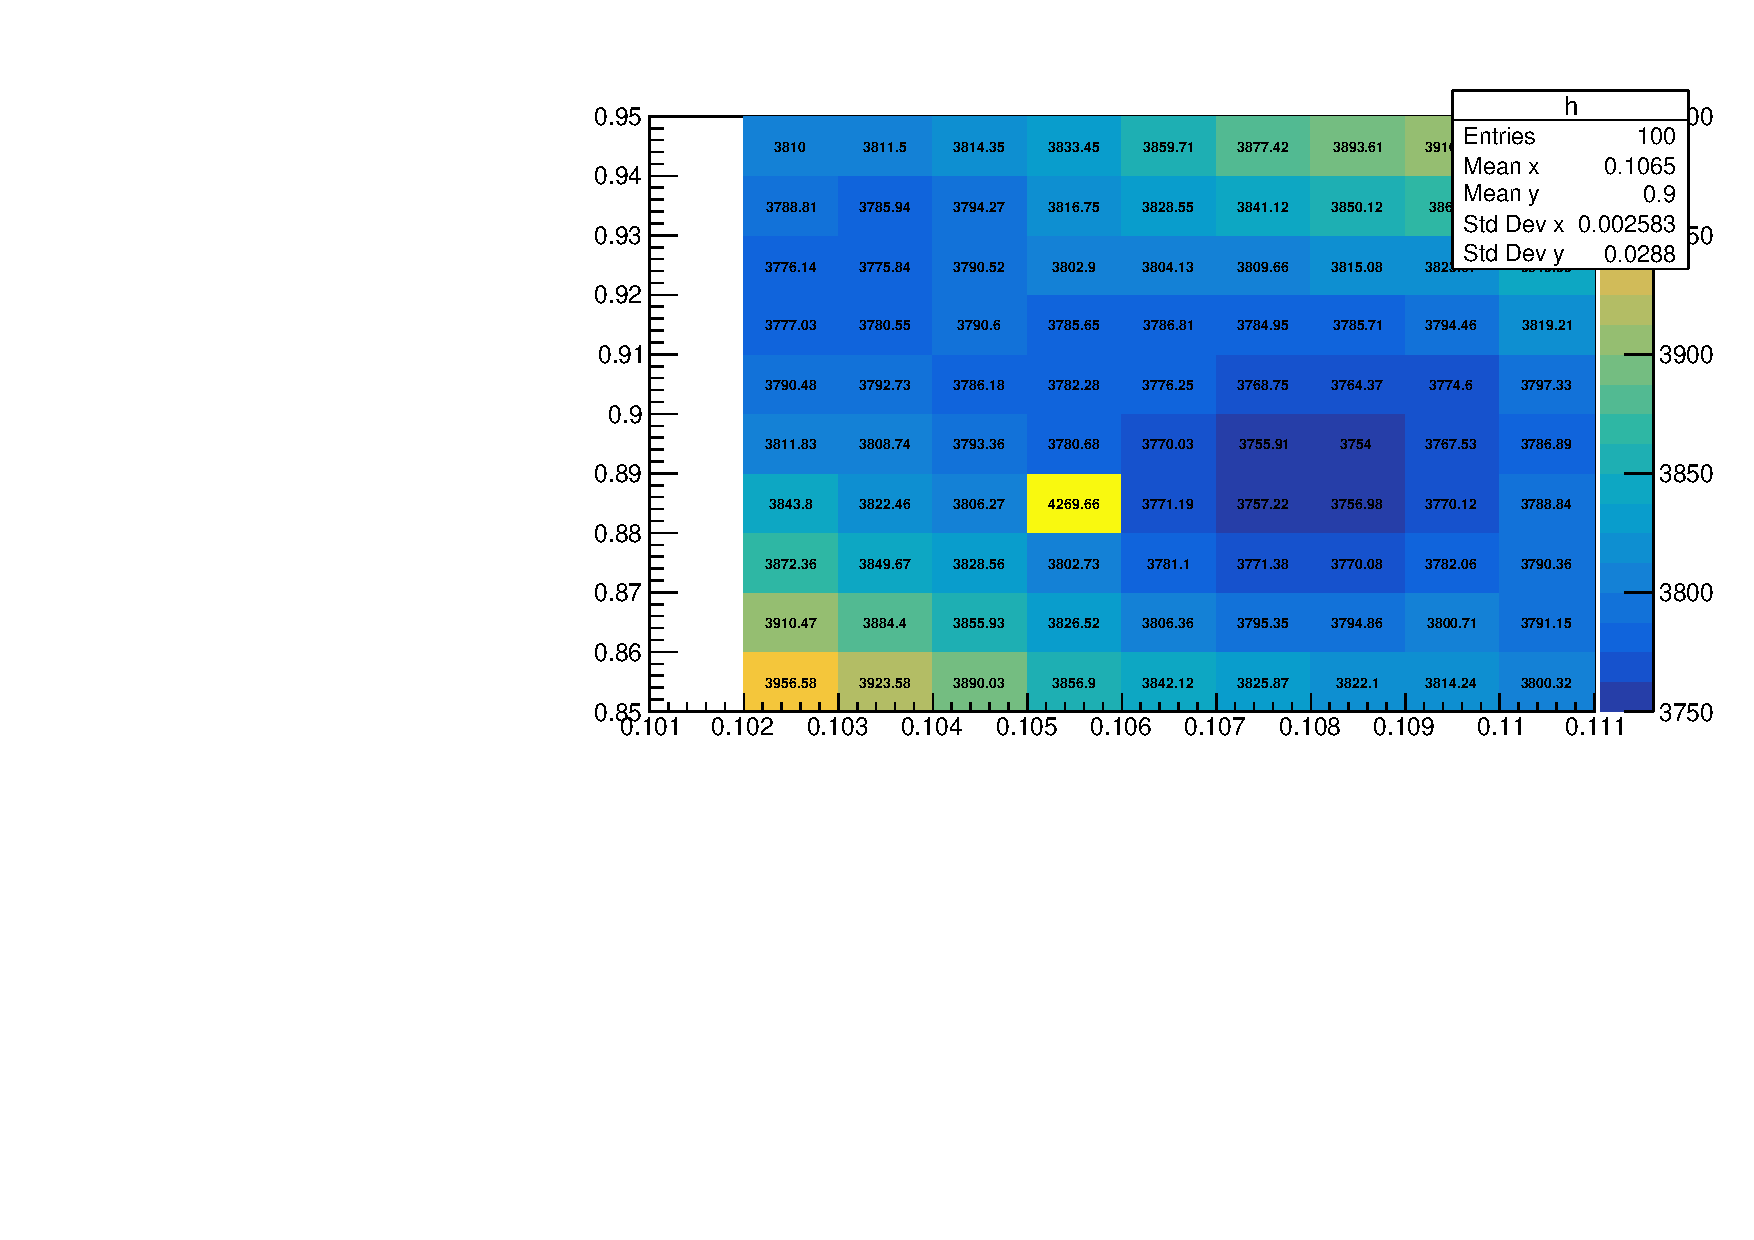
\includegraphics[width=80mm]{figures/chi2.pdf}
\caption{$\chi^2$ distribution of different Birk's constants and Cherenkov efficiency.}
\label{fig:chi2}
\end{figure}

\section{Conclusion/Next}
\subsection{Conclustion}
BLAH (NO STRONG CONCLUSION YET.)
\subsection{Next}
\begin{itemize}
    \item Check the best-fit values with single segment response.
    \item Check different ZLE's impact on the fit.
    \item Draw a figure with $E_{model}/E_{rec}$.
    \item Check the best-fit values with reactor off n-H and other sources.
\end{itemize}

%\newpage
%\appendix
%\section{...}
%\label{sec:resources}


%\newpage
%\bibliography{}
%\bibliography{citations.bib}{}

\end{document}